\chapter{Creating an Application}
\label{cha:createApplication}

	\section{Introduction}
		The previous chapters were all about \textit{STORM}. This chapter should give
		you an overview of \emph{how to use} it. Even though it would be possible
		to create a new application in a relatively short time, we stay with our 
		order application example. This is not meant as a step by step guidance but
		as a ``not so short introduction to create an application with \textit{STORM}''.
		Some parts in this chapter have already been mentioned. They
		are repeated to put them in the context of creating a new application.
	
	\section{Starting a Design}
		In the case of the order application, the database design was already existing.
		Therefore, this has been taken as starting point. Usually, the starting
		point would be a domain model but it makes not much of a difference. The
		database design is shown in Figure \ref{fig:dbDesign}. The corresponding
		conceptional domain model is shown in Figure \ref{fig:designConceptModel}.
		The domain model looks essentially the same as the database model.
		This is because every domain object will be mapped to a table in
		the database. The design of an application is always the starting point
		and should be done carefully.
		
		Our order application is not very difficult to explain. It contains
		persons with addresses. One person can have multiple addresses. But an
		address in turn belongs always to only one person. Furthermore, a person
		can have multiple orders. An order contains order details which describe
		the order and its details like price and quantity. A product then
		is related to an order detail.
			
		\begin{figure}[htb]
			\begin{center}
				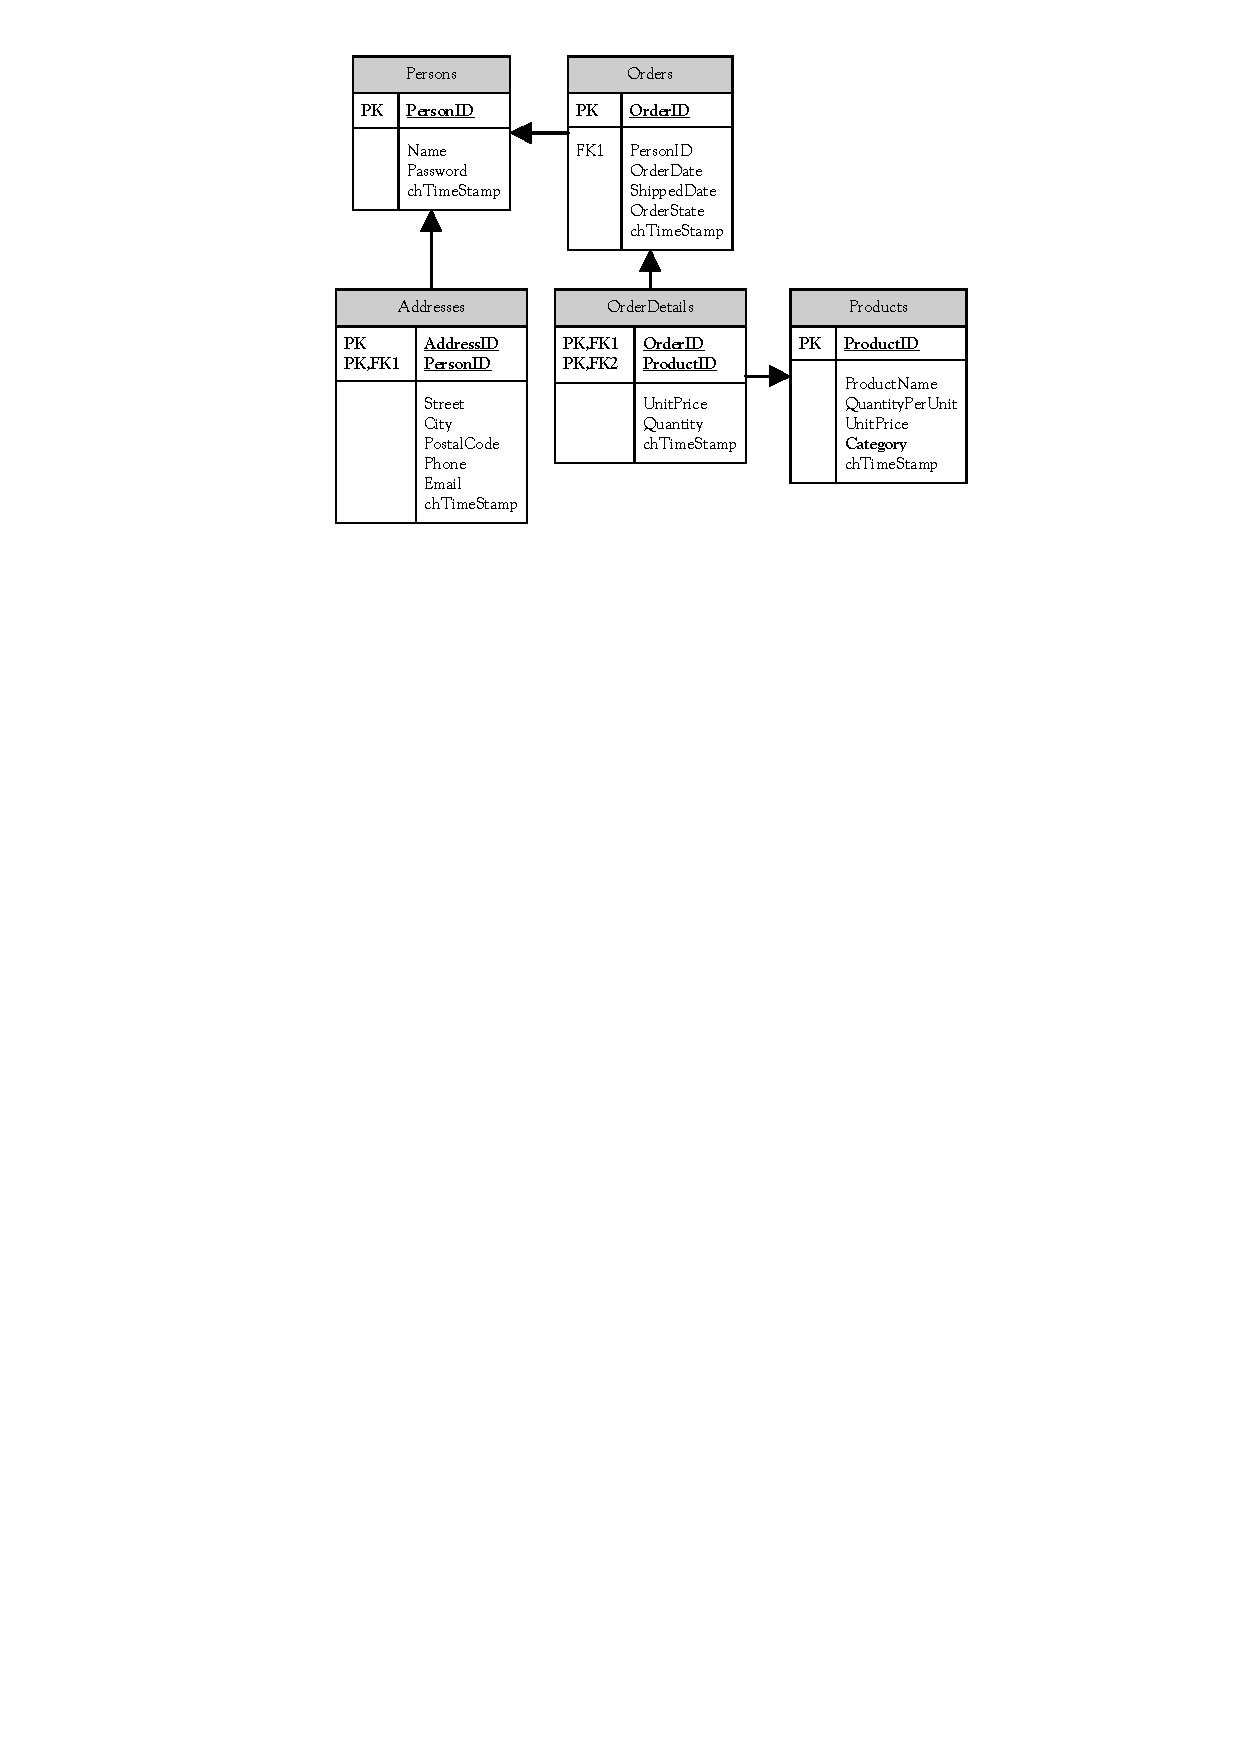
\includegraphics{./files/inc/figures/DbDesign}
				\caption{\label{fig:dbDesign}Database Design}
			\end{center}
		\end{figure}

		\begin{figure}[htb]
			\begin{center}
				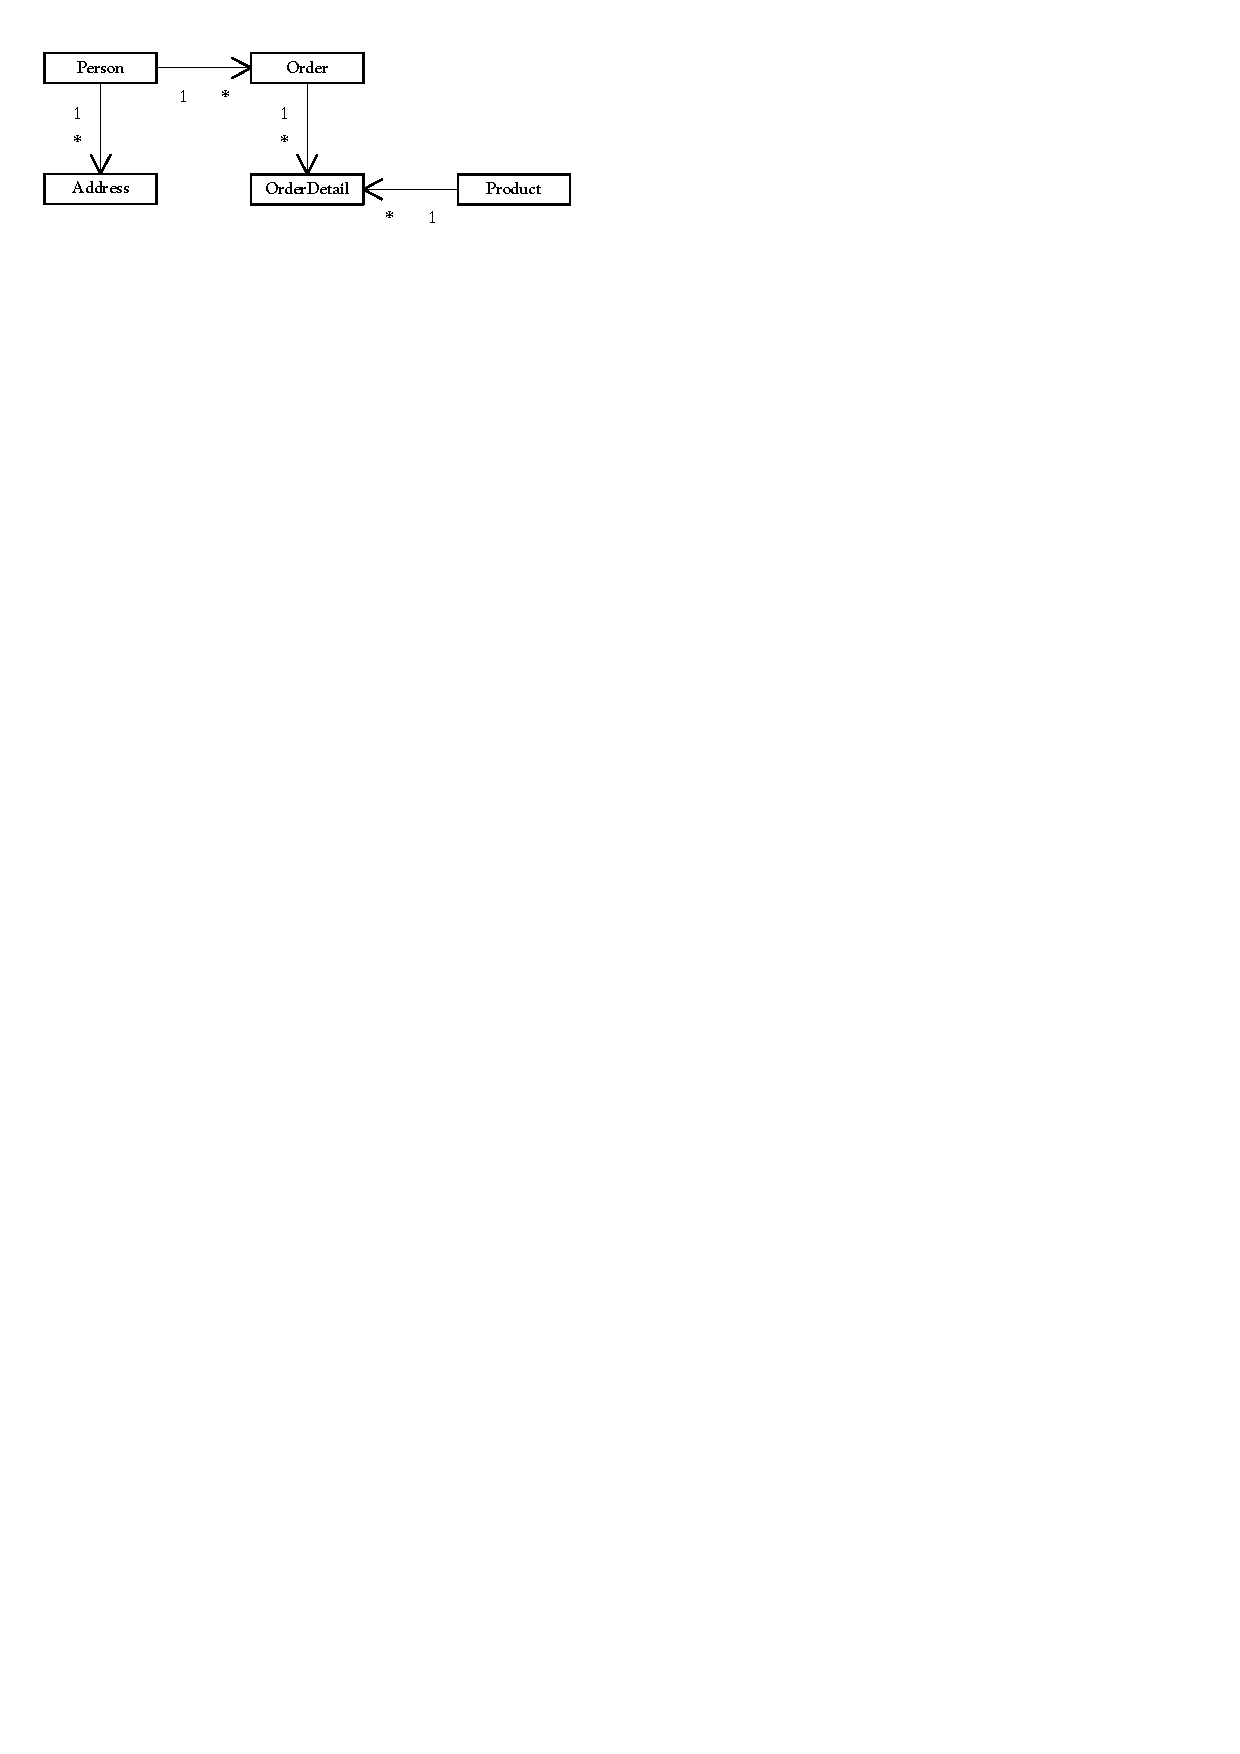
\includegraphics{./files/inc/figures/DesignConceptModel}
				\caption{\label{fig:designConceptModel}Conceptional Domain Model}
			\end{center}
		\end{figure}
		
	\section{Preparation}
		In order to work with \textit{STORM}, some preliminary work needs to be done.
		Namely that is to make the ImplGen and MapperGen templates available for the current
		project. This means, they must exist on the file system. Where to put them is
		the decision of the developer. The templates can be references by providing
		the full path. We decided to place the templates in a folder in the current project.
		The next step is to add a reference to the	new project. This reference must point to 
		the \textit{STORM} dll file. And last, CodeSmith \footnote{\url{http://www.ericjsmith.net/codesmith/}}
		must be installed. Thats it.
	
	\section{Writing abstract Classes}
		When all the design and preparation has been finished, it is time for \textit{STORM} to
		come into play. The first step is to write an abstract classes for each class of the
		domain model. In our case this means to write an abstract class for \verb~Person~,
		\verb~Address~, \verb~Order~, \verb~OrderDetail~ and \verb~Product~. It is very
		important to write these classes carefully. Listing \ref{lst:abstractOrderDetail}
		shows the abstract class \verb~OrderDetail~. 
		
		\begin{lstlisting}[language={[Sharp]C},caption=Defining OrderDetail as abstract class.,
		label=lst:abstractOrderDetail]
[Table("Orders", true),
VersionField("chTimestamp"),
GenerateCode]
public abstract class Order : DomainObject
{
	[Factory]
	public abstract class OrderFactory
	{
		public abstract Order createOrder(
			[ParameterDef("Person")] Person person,
			[ParameterDef("OrderDate")] DateTime orderDate,
			[ParameterDef("ShippedDate")] DateTime shippedDate,
			[ParameterDef("OrderState")] String orderState);
	}

	[Finder]
	public abstract class OrderFinder
	{
		public abstract IList findByOrderDate(
			[ParameterDef("OrderDate")] DateTime orderDate);
		public IList findOrderedBetween(DateTime startDate, DateTime endDate)
		{
			return new ArrayList();
		}
		public IList findShippedBetween(DateTime startDate, DateTime endDate)
		{
			return new ArrayList();
		}
	}

	[Column("OrderID"),
	PrimaryKey]
	public abstract int OrderId {get;}

	[Column("PersonID"),
	ToOne(typeof(Person), "PersonId")]
	public abstract Person Person {get; set;}

	[Column("OrderDate")]
	public abstract DateTime OrderDate {get; set;}
	
	[Column("ShippedDate")]
	public abstract DateTime ShippedDate {get; set;}
	
	[Column("OrderState")]
	public abstract string OrderState {get; set;}

	[ToMany(typeof(OrderDetail), "Order")]
	public abstract IList OrderDetails {get;}
	
	[Adder("OrderDetails", "Order")]
	public abstract void addOrderDetail(OrderDetail od);

}
		\end{lstlisting}
		
		All other abstract classes must be defined analogical to this one. Additional
		methods can also be defined in this abstract class. They are defined without
		custom attributes. Such methods are ignored by the process of code
		generation.
		
		If all abstract classes are implemented, the main work of writing the core
		application is done.		
		
	\section{Configuration Files}
		The next step is to generate all domain and mapper implementations. This is done using 
		CodeSmith's Custom Tool. In order to use CodeSmith from within the Visual Studio .NET, 
		an XML configuration file must exist. In this configuration file are all information
		that CodeSmith needs to generate the code. It would be possible to have just
		two XML files per project, one for the ImplGen and one for the MapperGen template. This
		would generate all domain implementation code in one file and all mapper code in another.
		We decided to split the code and make two files for each abstract class.
		A Sample of such an XML file is given in Listing \ref{lst:xmlConfigOrder}. That is an
		XML configuration file for an \verb~Order~ class. Out of this, the domain object
		implementation will be generated. The same file is needed for the mapper
		implementation. The only difference is that the template would not be ImplGen but
		MapperGen (see line 24). Depending on the application, also different namespace
		imports would be needed. The generated file has the same name as the
		XML file, e.g. if we name the XML file \verb~OrderImpl.xml~, the output file name
		would be \verb~OrderImpl.cs~.
		
		\begin{lstlisting}[float=htb,language={[Sharp]C},caption=CodeSmith Configuration File,
		label=lst:xmlConfigOrder]
<?xml version="1.0" encoding="utf-8" ?> 
<codeSmith>
<namespace>HsrOrderApp.BusinessLayer.DomainModelImpl</namespace>
	<imports>
		<import namespace="System" />
		<import namespace="System.Collections" />
		<import namespace="System.Reflection" />
		<import namespace="Storm.Lib" />
		<import namespace="Storm.Attributes" />
		<import namespace="HsrOrderApp.BusinessLayer.DomainModel" />
	</imports>
	<propertySets>
		<propertySet>
			<property name="assemblyLoader">
				<AssemblyLoader>
					<SourceAssembly>
						C:\HsrOrderApp\BusinessLayer\bin\Debug\BusinessLayer.dll
          </SourceAssembly>
					<ClassName>Order</ClassName>
				</AssemblyLoader>
			</property>
		</propertySet>
	</propertySets>
	<template path="..\Templates\ImplGen.cst" />
</codeSmith>
		\end{lstlisting}
				
	
	\section{Generating the Code}
	
		There are two ways to generate code without the CodeSmith GUI. You can choose between 
		a command line tool and the possibility to 
		integrate the generation into Microsoft Visual Studio .NET. Both take 
		the settings from an xml file as described in the last section.
		
		The command line tool is very useful for creating makefiles. The integrated
		tool is easy to use while writing code. Both methods can be used and both work.

		To run the generation of code from within the Visual Studio you have to add the xml 
		configuration file to the Visual Studio project. Then you have to set the 
		property \verb~Custom Tool~ to \verb~CodeSmithGenerator~ as shown in Figure 
		\ref{fig:vsdotnetCustomTool} on the right.
		
		The \verb~Build Action~ field has to be set to \verb~Content~. This causes Visual Studio 
		to execute the generation every time the content of the xml file has changed. The generation 
		of the code can also be initiated by right clicking the xml file and select 
		\verb~Run Custom Tool~.
		
		\begin{figure}[thb]
			\begin{center}
				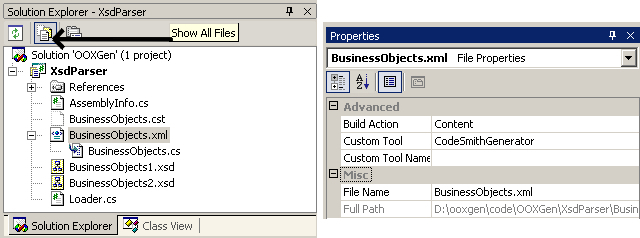
\includegraphics[width=11cm]{./files/inc/figures/codesmithVsdotnet}
				\caption{\label{fig:vsdotnetCustomTool}Visual Studio .NET integration}
			\end{center}
		\end{figure}
		
		If the option \emph{Show All Files} (see Figure \ref{fig:vsdotnetCustomTool}) is 
		turned on, the generated file is displayed as a child of the xml file.
	
	\section{Working with the Application}
		Now, everything is created and ready to use. To actually use the code we need a
		client application which uses the generated classes. This can be of any
		complexity and size. For this example, we use a very basic console
		application. Listing \ref{lst:sampleApplication} shows the code of the test method.
		First, and important, the program class the registry's \verb~init()~ method.
		Parameters are the running program (this) and the host and name of the
		database to be used (line 3).
		After initialisation, the application searches all persons in the database.
		Next, a specific person is searched. That is, the person with the Id 2. All
		orders for this person are wrote to the console. To finish the sample
		program, a new order for this person is created. This order is added to 
		the person and changed afterwards.
		
		After everything has been done, a commit on the unit of work is called.
		This executes all operations on the database.
		
		\begin{lstlisting}[language={[Sharp]C},caption=Sample console application,
		label=lst:sampleApplication]
public void test()
{
	Registry.Instance.init(this, "localhost", "OrderApplication");

	IList persons = (Person.PersonFinder)Registry.Instance.
		getFinder(typeof(Person)).findAll();

	Person person = (Person)Registry.Instance.
		getFinder(typeof(Person)).findById(new Key(new object[] {2}));
	
	foreach(Order order in person.Orders)
	{
		Console.WriteLine(order);
	}

	Order order = ((Order.OrderFactory)Registry.Instance.
		getFactory(typeof(Order))).
		createOrder(person, new DateTime(2003, 12, 1), null, "");
		
	person.addOrder(order);

	order.ShippedDate = DateTime.Today;
	
	UnitOfWork.Instance.commit();
}
		\end{lstlisting}
		
		Although this is a very simple application, it should give an impression how
		fast an application can be build using \textit{STORM}. A great advantage
		of using a generative programming technique is, that even if an application
		becomes larger, there is not much extra work to do. The only thing which 
		needs to be done is to implement another abstract class.
		